\documentclass[12pt, a4paper, russian]{article}
\usepackage[margin=2cm]{geometry}
\usepackage[T2A]{fontenc}
\usepackage[utf8]{inputenc}
\usepackage[english,russian]{babel}
\usepackage{amsmath}
\usepackage{subfig}
\usepackage{caption}
\usepackage[compress]{cite}
\usepackage{graphicx}
\usepackage{xcolor}
\usepackage{algorithm}
\usepackage{algpseudocode}
\usepackage{enumitem}
\usepackage{multirow}
\usepackage{booktabs}
\usepackage{titling}
\usepackage[hidelinks]{hyperref}
\usepackage{setspace}
\singlespacing

% To prevent LaTeX from hyphenating
\tolerance=1
\emergencystretch=\maxdimen
\hyphenpenalty=10000
\hbadness=10000

\makeatletter \renewcommand*{\ALG@name}{Алгоритм} \makeatother


%%%%%%%%%%%%%%%%%%%%%%%%%%%%%%%%%%%%%%%%%%%%%%%%%%
\begin{document}

%%%%%%
%%%%%% Информация на английском языке
%%%%%%

\title{Global optimization algorithm using decision trees to find local extrema \thanks{The work was supported by the oneAPI Center of Excellence, by the Ministry of Science and Higher Education of the Russian Federation (project no. 0729-2020-0055), and by the Research and Education Mathematical Center (project no.  075-02-2021-1394).}}

\author{D.~I.~Silenko, I.~G.~Lebedev\\
	\small{Lobachevsky State University of Nizhny Novgorod, 603022, Nizhny Novgorod, Russia}
}
\date{}
\maketitle

\begin{small}
\textbf{Abstract:} The paper considers the solution of multidimensional global optimization problems using decision trees to identify areas of attraction of local minima. The local method is used for local refinement and is designed to speed up the convergence of the algorithm. The desired function satisfies the Lipschitz condition with an unknown constant. To confirm the theory, computational experiments were presented demonstrating acceleration when solving a series of test problems.

\textbf{Key words:} Global optimization, multiextremal functions, parallel computing, decision tree.
\end{small}

% References
\renewcommand{\refname}{References}
\bibliographystyle{IEEEtran}
\bibliography{articleEng}



%%%%%% 
%%%%%% Информация на русском языке
%%%%%%
\emptythanks
\title{Алгоритм глобальной оптимизации, использующий деревья решений для выявления локальных экстремумов\thanks{Работа выполнена при финансовой поддержке Министерства науки и высшего образования РФ (проект № 0729-2020-0055) и научно-образовательного математического центра “Математика технологий будущего” (соглашение № 075-02-2021-1394).}}

\author{Д. И. Силенко, И. Г. Лебедев\\
	\small{Нижегородский государственный университет им. Н. И. Лобачевского, 603022, Н.Новгород, Россия} 
}
\date{}
\maketitle

УДК 004.222+004.272.25

\vspace{\baselineskip}

\begin{small}
\textbf{Аннотация:} В работе рассматривается решение задач многомерной глобальной оптимизации с применением деревьев решений для выявления областей притяжения локальных минимумов. Локальный метод используется для локального уточнения и призван ускорить сходимость алгоритма. Искомая функция удовлетворяет условию Липшица с неизвестной константой. Для подтверждения теории были приведены вычислительные эксперименты, демонстрирующие ускорение при решении серии тестовых задач.

\textbf{Ключевые слова:} глобальная оптимизация, локальная оптимизация, многоэкстремальные функции, деревья решений.
\end{small}


\section{Введение}

При поиске глобального минимума функции можно придерживаться различных алгоритмов: от основанных на идее случайного поиска \cite{fio_bib1, fio_bib2, fio_bib3}, до детерминированных алгоритмов, гарантирующих сходимость к глобальному минимуму \cite{fio_bib4, fio_bib5, fio_bib6}. Поскольку в реальных задачах глобальной оптимизации каждое вычисление значения функции представляет собой весьма трудоемкую задачу, необходимо уменьшить количество таких операций. Этого можно добиться целенаправленным выбором вариантов в процессе поиска оптимального решения. На этой идее основывается алгоритм глобального поиска (АГП). В данной работе мы попробуем объединить АГП и метод локальной оптимизации (метод Хука-Дживса) с помощью деревьев решений, с целью уменьшить количество проводимых итераций, а вместе с этим и количество вычислений целевой функции.

Алгоритмы поиска локального экстремума предназначены для определения лишь одного из локальных экстремумов на множестве допустимых решений, в котором целевая функция принимает максимальное или минимальное значение. При их построении могут использоваться как детерминированный спуск в область экстремума, так и случайный поиск. Среди детерминированных различают методы нулевого порядка и градиентные (1-го и 2-го порядка).

Для того, чтобы понять, в какой момент лучше всего запускать локальный метод, мы используем алгоритм на основе деревьев решений. Мы накапливаем определенное число точек и лишь когда их станет достаточно начинаем обработку. Эти полученные точки мы используем для тренировки деревьев решений и предсказания по нему. Предсказание позволяет нам получить кусочно-линейную аппроксимацию по этому дереву. После чего мы рассматриваем уже полученную по дереву аппроксимацию. Проверяем значения соседних точек к той, которую считаем подозрительной на минимум, и оцениваем попали мы в область притяжения локального минимума или нет. 

\section{Постановка задачи}

Рассмотрим задачу поиска глобального минимума функции $\varphi(y)$ в гиперинтервале $D=\{ y\in\ R^N:\ a_i\le\ y_i\le\ b_i,\ 1\le\ i\le\ n \}$ При этом будем предполагать, что функция удовлетворяет условию Липшица с априори неизвестной константой $L$. Что соответствует ограниченности изменения значений функции при ограниченной вариации аргумента. Это предположение можно интерпретировать (применительно к прикладным задачам) как отражение ограниченности мощностей, порождающих изменения в моделируемой системе. 




\begin{equation} \label{sec:problem}   
\varphi(y^*) = min\{\varphi(y):y\in D\}, D = \{y \in R^N : a_i \leq y_i \leq b_i, 1 \leq i \leq N \},
\end{equation}
где $a,b \in R$ --- заданные векторы.


\begin{displaymath}
|\varphi(y_1)-\varphi(y_2)|\leq L\parallel y_1-y_2 \parallel
,y_1,y_2 \in D, 0<L< \infty.
\end{displaymath}




Численное решение задачи (\ref{sec:problem})   сводится к построению оценки $ y_k^\ast\in\ D$ , отвечающей некоторому понятию близости к точке $y^\ast$ (например, ${||y^\ast-y}_k^\ast||\le\ \varepsilon$, где $\varepsilon\geq0$ есть заданная точность) на основе конечного числа $k$ вычислений значений оптимизируемой функции. Относительно класса рассматриваемых задач предполагается, что оптимизируемая функция $\varphi(y)$ может быть задана не аналитически, в виде формулы, а алгоритмически, как результат работы некоторой подпрограммы или библиотеки.

Задачи многоэкстремальной оптимизации имеют существенно более высокую трудоемкость решения по сравнению с другими типами оптимизационных задач, т.к. глобальный оптимум является интегральной характеристикой решаемой задачи и требует исследования всей области поиска. Как результат, поиск глобального оптимума сводится к построению некоторого покрытия (сетки) в области параметров, и выборе наилучшего значения функции на данной сетке. Вычислительные затраты на решение задачи растут экспоненциально с ростом размерности.


\section{Многомерный алгоритм глобального поиска}

Основная идея данного подхода заключается в том, что минимизируемая функция рассматривается как реализация некоторого случайного процесса. Решающие правила алгоритма конструируются таким образом, что очередная итерация проводится в точке глобального минимума математического ожидания значений функции. Эта точка записывается в список известных значений и итерации повторяются. Так происходит до тех пор, пока не достигнут один из выбранных критериев остановки: расстояние между точками отрезка не становится меньше заданного значения или новые точки не попадают в окрестность истинного глобального минимума. Еще одним вариантом остановки работы алгоритма является достижение установленного максимума возможных итераций. \cite{fio_bib10}

При решении многомерных задач применяется редукция размерности (т.е. сведение многомерной задачи к эквивалентной одномерной) с использованием кривых Пеано. Они позволяют свести многомерную задачу минимизации в области $D$  к одномерной задаче минимизации на отрезке $[0, 1]$

\begin{equation*}
\phi({y(x}^\ast))\ =\ min\{\phi(y(x)):\ x\epsilon[0,\ 1]\}
\end{equation*}
где функция  удовлетворяют уже равномерному условию Гельдера
\begin{equation*}
\left|\phi (y \left(x_1\right))- \phi (y \left(x_2\right)\right )|\le\ H\left|x_1-x_2\right|^\frac{1}{N},\ x_1,\ x_2\epsilon[0,1]		
\end{equation*}

Поэтому, не ограничивая общности, можно рассматривать минимизацию одномерной функции $f(x)\ =\ \phi(y(x)), \ x\epsilon [0,1]$, удовлетворяющей условию Гельдера.

Схема алгоритма:

На подготовительном шаге параллельно проводятся $p$ поисковых испытаний в произвольных внутренних точках $x^1, ...,x^p$ отрезка $[0,1]$, что соответствует первой итерации  алгоритма. 

Если выполнено $n\geq1$ итераций, которым соответствуют $k=k(n)$ проведенных поисковых испытаний в точках $x^i, 1\leq i\leq k$, то точки $x^{k+1},\ldots,x^{k+p}$ испытаний следующей $(n+1)$-й итерации будут определять следующим образом.

\begin{enumerate}

\item  Перенумеровать (нижним индексом) точки ранее проведенных испытаний $x^i, 1\leq i\leq k$, а также граничные точки отрезка [0,1] в порядке возрастания координаты:
 \begin{equation}
\label{agp1_sort}
	0=x_0<\ x_1<\ ...\ <x_{k+1}=1.
	\end{equation}
	и сопоставить им значения $z_i=f(x_i)$. 
	
\item  Вычислить текущие нижние оценки $M$ неизвестной константы Гельдера $H$:
 \begin{equation}
\label{agp2_mu}
	\mu=max\left\{\frac{|z_i-z_{i-1}|}{{{(x}_i-x_{i-1})}^{1/N}},\ i=1,\ldots,k\right\},\ M=\ \left\{\begin{matrix}r\mu,\ \mu>0,\\1,\ \mu=0,\\\end{matrix}\right.\
	\end{equation}
где $r>1$ --- заданный параметр алгоритма.
   
\item  Для каждого интервала $(x_{i-1},x_i), 1\leq i\leq k+1,$ вычислить величину $R(i)$, называемую \textit{характеристикой} интервала, в соответствии с формулами
\begin{equation}
\label{agp3_R1}
R(1)=2\Delta_1-4\dfrac{z_1}{M}, \; R(k+1)=2\Delta_{k+1}-4\dfrac{z_k}{M},
\end{equation}
\begin{equation}
\label{agp3_Ri}
R(i)=\Delta_i+\dfrac{(z_i-z_{i-1})^2}{M^2\Delta_i}-2\dfrac{z_i+z_{i-1}}{M},1<i<k+1,
\end{equation}
где \(\Delta_i=(x_i-x_{i-1})^\frac{1}{N}\).
   
\item   Упорядочить характеристики $R\left(i\right),\ 1\leq i \leq k+1,$ в порядке невозрастания 
\begin{equation}
\label{agp4_R_sort}
	R\left(t_1\right)\geq\ R\left(t_2\right)\geq...\geq\ R\left(t_k\right)\geq\ R(t_{k+1}),\ 
\end{equation}	
и выбрать интервал с номерами $t$, с наибольшими значениями характеристики.

\item  В выбранном интервале вычислить точку $x^{k+1}$, в соответствии с формулами
\begin{equation}
\label{agp5_x1}
	x^{k+j}=\frac{x_{t_j}+x_{t_j-1}}{2},\ t_j=1,\ t_j=k+1,
\end{equation}	
	\begin{equation}
\label{agp4_xi}	
	x^{k+1}=\frac{x_{t_j}+x_{t_j-1}}{2}-sign\left(z_{t_j}-z_{t_j-1}\right)\frac{1}{2r}\left[\frac{\left|z_{t_j}-z_{t_j-1}\right|}{\mu}\right]^N,\ 1<t_j<k+1.
\end{equation}	

\end{enumerate}

Отметим, что в прикладных оптимизационных задачах процесс проведения испытания является, как правило, значительно более трудоемким по сравнению с работой вычислительных правил алгоритма.

Алгоритм останавливает свою работу в случае, если значения $t$ из (\ref{agp4_R_sort}) выполняется условие \(\Delta_{t_j} < \varepsilon\). Данный критерий остановки (наряду с обычным для итерационных методов критерием, ограничивающим число выполненных итераций) используется в задачах оптимизации, в которых точка глобального минимума $x^*$ заранее неизвестна. 
	 
При решении тестовых задач, в которых точка глобального минимума $x^*$ является  известной, можно использовать также и критерий остановки по попаданию в окрестность глобального минимума. В этом случае метод прекращает работу, если если хотя бы для одного значения $t_j,\ 1\le\ j\le\ p$ из (\ref{agp4_R_sort}) выполняется условие $\left|x_{t_j}-\ x^\ast\right| < \varepsilon.$
	
В качестве итоговой оценки глобально-оптимального решения рассматриваемой задачи выбираются значения 
\begin{equation}
f_k^*=\min_{1\leq i \leq k}f(x_i), \; x_k^*=arg \min_{1\leq i \leq k}f(x_i).
\end{equation}



Обоснование данного способа организации вычислений см. в \cite{fio_bib20}. Модификации, учитывающие наличие ограничений-неравенств в задаче, а также информация о производной целевой функции, представлены в \cite{fio_bib12, fio_bib9, fio_bib11}.


\section{Метод Хука-Дживса}

Метод Хука–Дживса --- это комбинация исследующего поиска по направлениям и поиска по образцу \cite{fio_bib14, fio_bib15}.



Исследующий поиск определяется следующим образом: 
\begin{enumerate}
\item	Определяется значение шага (оно различно для каждого направления координат и может измениться во время поиска). 
\item	Шаг поиска считается успешным, если значение целевой функции в контрольной точке не превышает значение исходной целевой функции. 
\item	В противном случае нужно вернуться к предыдущему пункту и сделать шаг в обратном направлении. 
\item	После перебора всех N координат исследовательский поиск заканчивается. Полученная точка называется базовой точкой.
\end{enumerate}




Что касается поиска по образцу, то он заключается в реализации шага из найденной в ходе исследующего поиска базовой точки вдоль прямой, соединяющей ее с предыдущей базовой точкой. Величина этого шага определяется задаваемым заранее параметром.

\begin{figure}[!h]
	\begin{center}
		\begin{minipage}[h]{0.8\linewidth}
			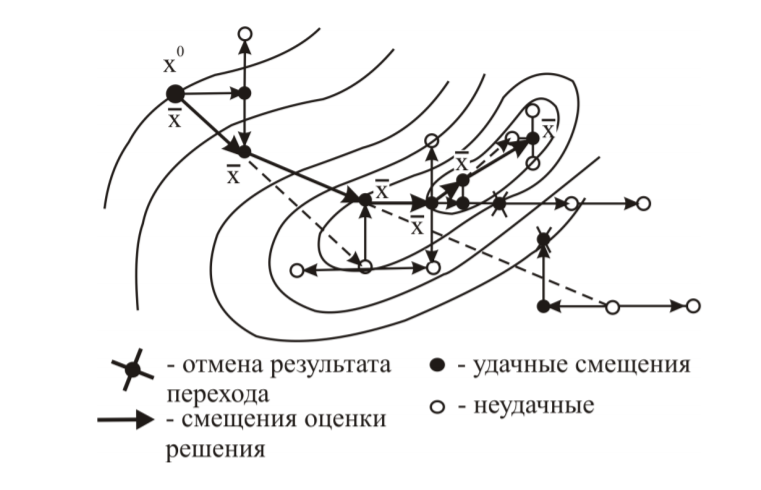
\includegraphics[width=1\linewidth]{figure/fig1.png}
			\caption{Пример итераций алгоритма Хука-Дживса} %% подпись к рисунку
			\label{fig:fig1}
		\end{minipage}
	\end{center}
\end{figure}	

\section{Деревья решений}

Деревья решений --- это метод автоматического анализа больших массивов данных, который применяется в машинном обучении. Деревья решений представляет собой бинарное дерево (дерево, в котором каждый не листовой узел имеет два дочерних узла). Его можно использовать как для решения задач классификации, так и для регрессионных задач. При решении задач классификации, каждый лист дерева помечается меткой класса, при этом несколько листьев могут иметь одну и ту же метку. В случае построение регрессии, каждому листу дерева присваивается константа, как следствие  получаемая функция аппроксимации является кусочно-постоянной.

Процедура прогнозирования по дереву решения начинается с корня. От каждого не листового узла процедура идет влево или вправо на основании значения некоторой переменной, индекс которой хранится в наблюдаемом узле. Возможны следующие переменные:
Упорядоченные переменные, значения которых сравнивается с порогом (который также хранится в узле). Если значение меньше порога, процедура идет влево. В противном случае --- вправо.
Категориальные переменные --- значение дискретной переменной проверяется на предмет того, принадлежит ли оно определенному подмножеству значений (также хранящемуся в узле) из набора допустимых величин. Если принадлежит, то идем влево. В противном случае --- вправо. 
Как только алгоритм достигает конечного узла, в качестве ответа процедуры прогнозирования выбирается значение, присвоенное этому узлу. 

В нашем случае дерево решений строит функцию $\varphi(y)$ кусочно постоянную аппроксимацию$\varphi(y)$  в многомерном пространстве, обозначим как $z' = \psi(y)$ значение вычисленное по decision tree в точке $y$.

При реализации алгоритма  решения задач многомерной глобальной оптимизации с применением деревьев решений для выявления областей притяжения локальных минимумов нами были использованы  деревья решений из библиотеки OpenCV (это библиотека алгоритмов компьютерного зрения, обработки изображений и численных алгоритмов общего назначения с открытым кодом). Подробнее с  деревьями решений можно ознакомиться в \cite{fio_bib16}


\section{Объединение локального метода и АГП в случае многомерных задач}

В текущем разделе приведем подробное описание того, как использовать деревьев решений в многомерном случае. В процессе работы АГП необходимо определить, стоит ли использовать текущую точку, в качестве стартовой для локального метода или нет. Для этого можно осмотреть соседние точки испытания и если среди них нет ни одной такой, значение функции в которой меньше, чем в текущей, то можно предположить, что мы находимся в области притяжения локального минимума и можно запустить локальный метод, чтобы быстрее сойтись к минимуму. Использование проекций многомерных точек на одномерный отрезок после редукции размерности (то, что позволяют сделать кривые Пеано) нам для этих целей не подойдут по нескольким причинам. Во-первых, функция после отображения сильно изменяется, один локальный минимум в многомерном пространстве может разделиться на множество минимумов после отображения. Во-вторых, после отображения мы можем потерять информацию о взаимном расположении точек исходной функции. Точки, расположенные близко в многомерном пространстве, могут оказаться на разных концах одномерного отрезка и наоборот).

%\begin{figure}[ht!]
%	\begin{center}
%		\begin{minipage}[h]{0.8\linewidth}
%			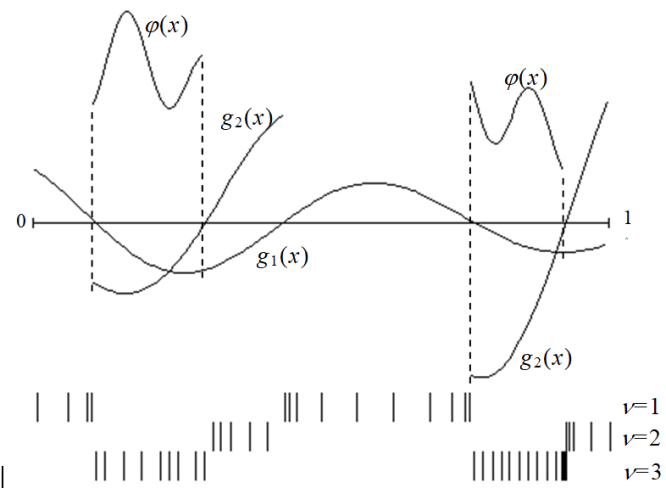
\includegraphics[width=1\linewidth]{figure/fig2.png}
%			\caption{Функция из генератора gkls до использования кривых Пеано} %% подпись к рисунку
%			\label{fig:fig2}
%		\end{minipage}
%	\end{center}
%\end{figure}	

%\begin{figure}[ht!]
%	\begin{center}
%		\begin{minipage}[h]{0.8\linewidth}
%			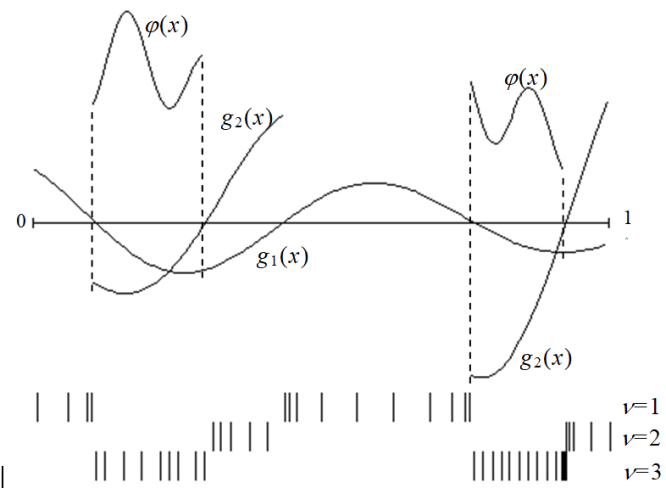
\includegraphics[width=1\linewidth]{figure/fig2.png}
%			\caption{Рисунок с двумерным деревом решений} %% подпись к рисунку
%			\label{fig:fig2_2}
%		\end{minipage}
%	\end{center}
%\end{figure}	


Поэтому мы будем работать именно с исходными точками. Однако определить соседние точки в многомерном пространстве достаточно трудоемко, и для этого мы будем использовать деревья решений. 

После проведения определенного числа испытаний (например, $100\ \ast\ N$), используем все накопившиеся точки для инициализации подходящей структуры данных и тренировки на ее основе дерева решений. Чтобы проще было определить соседние точки, мы построим равномерную сетку с определенным шагом по каждой из размерностей, после чего передадим эти точки на вход предсказанию по дереву. Теперь, имея равномерную сетку точек и зная значение функции в каждой из них, найдем ближайшую, с точки зрения евклидова расстояния, к исходной. Эта ближайшая точка является проекцией изначальной точки на равномерную сетку и что бы определить  ее соседей, достаточно  просто перебрать индексы соседей. К тому же поскольку дерево решений строит аппроксимацию исходной задачи (пусть и кусочно постоянную) мы можем оценить значение функции в тех областях, в которых испытания ранее не проводились.

При рассмотрении соседей необходимо учитывать следующее: если хоть один из соседей имеет значение функции меньшее, чем в текущей точке, то запуск локального метода не нужен; если какой-то из соседей имеет значение функции такое же, как в текущей, то его также необходимо проверить (найти всех его соседей и проверять их аналогично); и только в том случае, если все значения функций соседей больше (включая соседей равных точек) мы можем запускать локальный метод. Модифицированная версия алгоритма глобального поиска выглядит следующим образом:


\begin{enumerate}
	
	\item  Перенумеровать (нижним индексом) точки ранее проведенных испытаний $x^i, 1\leq i\leq k$, а также граничные точки отрезка [0,1] в порядке возрастания координаты:
	\begin{equation}
		\label{agp1_sort}
		0=x_0<\ x_1<\ ...\ <x_{k+1}=1.
	\end{equation}
	и сопоставить им значения $z_i=f(x_i)$. 
	
	\item  Вычислить текущие нижние оценки $M$ неизвестной константы Гельдера $H$:
	\begin{equation}
		\label{agp2_mu}
		\mu=max\left\{\frac{|z_i-z_{i-1}|}{{{(x}_i-x_{i-1})}^{1/N}},\ i=1,\ldots,k\right\},\ M=\ \left\{\begin{matrix}r\mu,\ \mu>0,\\1,\ \mu=0,\\\end{matrix}\right.\
	\end{equation}
	где $r>1$ --- заданный параметр алгоритма.
	
	\item  Для каждого интервала $(x_{i-1},x_i), 1\leq i\leq k+1,$ вычислить величину $R(i)$, называемую \textit{характеристикой} интервала, в соответствии с формулами
	\begin{equation}
		\label{agp3_R1}
		R(1)=2\Delta_1-4\dfrac{z_1}{M}, \; R(k+1)=2\Delta_{k+1}-4\dfrac{z_k}{M},
	\end{equation}
	\begin{equation}
		\label{agp3_Ri}
		R(i)=\Delta_i+\dfrac{(z_i-z_{i-1})^2}{M^2\Delta_i}-2\dfrac{z_i+z_{i-1}}{M},1<i<k+1,
	\end{equation}
	где \(\Delta_i=(x_i-x_{i-1})^\frac{1}{N}\).
	
	\item   Упорядочить характеристики $R\left(i\right),\ 1\leq i \leq k+1,$ в порядке невозрастания 
	\begin{equation}
		\label{agp4_R_sort}
		R\left(t_1\right)\geq\ R\left(t_2\right)\geq...\geq\ R\left(t_k\right)\geq\ R(t_{k+1}),\ 
	\end{equation}	
	и выбрать интервал с номерами $t$, с наибольшими значениями характеристики.
	
	\item  В выбранном интервале вычислить точку $x^{k+1}$, в соответствии с формулами
	\begin{equation}
		\label{agp5_x1}
		x^{k+j}=\frac{x_{t_j}+x_{t_j-1}}{2},\ t_j=1,\ t_j=k+1,
	\end{equation}	
	\begin{equation}
		\label{agp4_xi}	
		x^{k+1}=\frac{x_{t_j}+x_{t_j-1}}{2}-sign\left(z_{t_j}-z_{t_j-1}\right)\frac{1}{2r}\left[\frac{\left|z_{t_j}-z_{t_j-1}\right|}{\mu}\right]^N,\ 1<t_j<k+1.
	\end{equation}	

\item  Получить вычисленное  значение функции с процесса $j$, добавить новый trial $z_j = f(y(x_j))$, к множеству $V$. 

%X_k=\left\{x^1,x^2,\ldots,x^{k+p}\right\}


\item 	Если $ k\ <\ 100\ast\ N$, то вернуться к шагу 1.

%\item 	Если используем decision tree не впервые, то перейти к пункту 15.

\item Создаем decision tree по множеству $I_k$, получаем функцию аппроксимации  $\psi(y)$.



\item 	Если используем decision tree впервые, то строим равномерную сетку

\begin{displaymath}
	Y'=\{ y'\in\ R^N:\ a_i\le\  {y'_i}^k \le\ b_i,\ 1\le\ i\le\ N,\ 1\le k\le\ \sqrt[N]{300}  \}
\end{displaymath}

\item 	Вычисляем значения аппроксимации: $Z' = \{ z'=  \psi(y'), y' \in Y'\}$

\item Для всех точек $y'\in V$:

Находим точку $y'_q$ ближайшую  к $y'$,

Производим обход соседей $y'_q$ по описанному ранее принципу.

Если ни у одной соседней точки не нашлось значений функции меньших, чем в $y'_q$, то запускаем локальный метод.

Очищаем множество $V$.


\end{enumerate}

%На рисунке  (\ref{fig:fig2}) отображены линии уровней оптимизационной задачи с отображением текущих  точек испытаний, и на рисунке  (\ref{fig:fig2_2}) отображено соответствующее дерево решений. 


Все полученные результаты были добавлены в систему globalizer \cite{fio_bib18}.
Если говорить более конкретно, то была реализована объединенная схема с запуском локальных методов в нужный момент, для чего была внедрена система  построения дерева решений, равномерной сетки и прочих сопутствующих вычислений.  
Ниже приведена блок-схема того, как данная схема была объединена с АГП.

\begin{figure}[ht!]

	\begin{center}
		\begin{minipage}[h]{0.9\linewidth}
			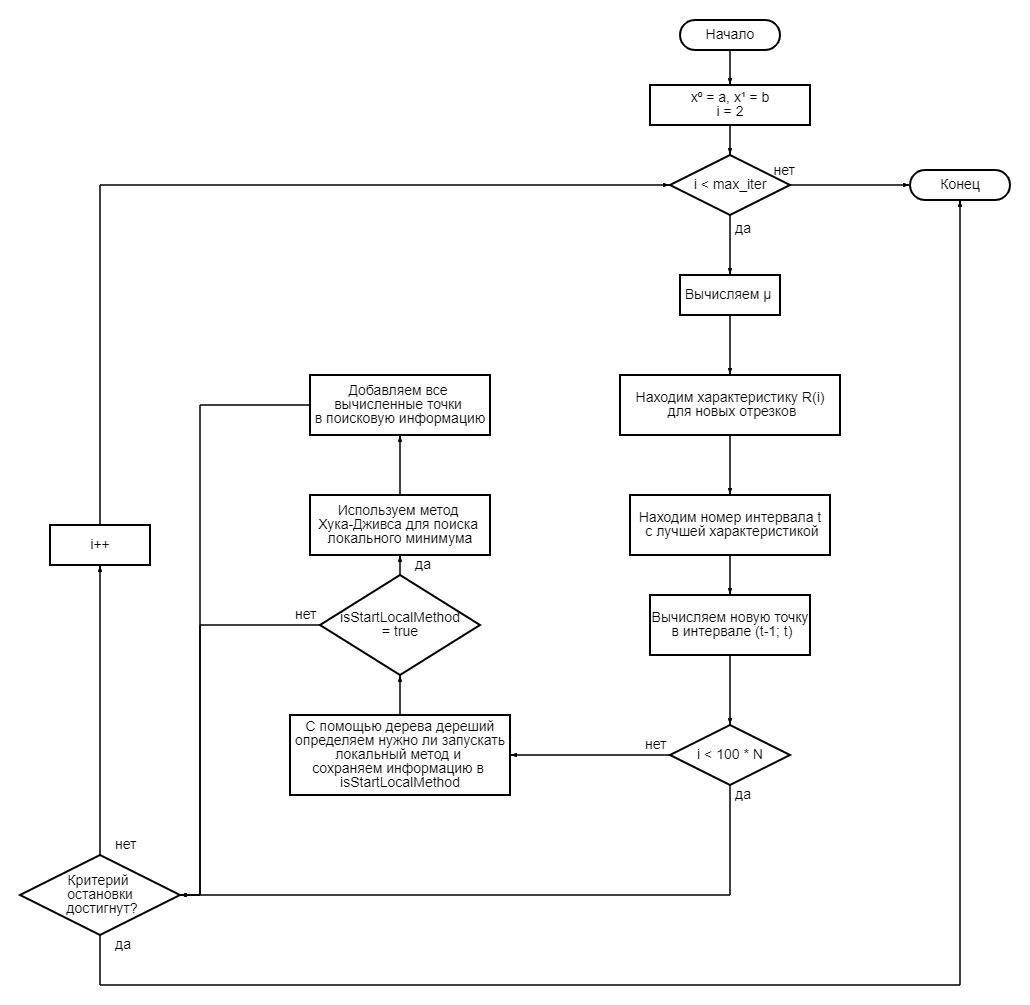
\includegraphics[width=1\linewidth]{figure/fig3.png}
			\caption{Блок-схема объединения АГП и метода Хука-Дживса с использованием дерева решений} %% подпись к рисунку
			\label{fig:fig3}
		\end{minipage}
	\end{center}
\end{figure}	

\section{Эксперименты}

Вычислительные эксперименты проводились на персональном компьютере со следующими характеристиками: Операционная система Windows 11,  Процессор: Intel(R) Core™ i5-8250U CPU @ 1.60 GHz, 12 Gb RAM.
В работе \cite{fio_bib13, fio_bib17} описан GKLS-генератор, позволяющий порождать задачи многоэкстремальной оптимизации с заранее известными свойствами: количеством локальных минимумов, размерами их областей притяжения, точкой глобального минимума, значением функции в ней и т.п.

В таблице \ref{tab:1} отражено среднее число итераций , которые выполнил метод при решении серии задач из данных классов. Символ «>» отражает ситуацию, когда не все задачи класса были решены каким-либо методом. Количество нерешенных задач указано в скобках.


\begin{table}[!ht]
    \caption{Среднее число итераций}
    \label{tab:1}
    \centering
    \begin{tabular}{|l|l|l|l|l|}
    \hline
        N & Problem class & DIRECT & DIRECTl & АГП  \\ \hline
        4 & Simple & >47282 (4) & 18983 & 11953  \\ \hline
        ~ & Hard & >95708 (7) & 68754 & 25263  \\ \hline
        5 & Simple & >16057 (1) & 16758 & 15920  \\ \hline
        ~ & Hard & >217215 (16) & >269064 (4) & >148342 (4)  \\ \hline
    \end{tabular}
\end{table}

Как видно из таблицы 1, АГП превосходит методы DIRECT и DIRECTl на всех классах задач по среднему числу итераций. 

Ниже приведены результаты сравнения двух алгоритмов – стандартного АГП и его объединение с методом Хука-Дживса, при использовании деревьев решений. Численное сравнение проводилось на классах функций Simple и Hard размерности 2, 3, 4 и 5 из \cite{fio_bib19}. Критерием остановки служило попадание точки испытания в эпсилон окрестность истинного глобального минимума. 
При этом измерялось не только среднее число проводимых испытаний, но и среднее число точек испытаний.

В таблице \ref{tab:2} представлено среднее количество итераций, и среднее число точек испытаний, проводимое двумя методами: алгоритмом глобального поиска (АГП) и объединением АГП и локального метода с использованием деревьев решений (Деревья решений) на задачах разной размерности ($N$) и разного класса (Класс задачи). Значение в скобках (если оно есть) показывает количество не решенных задач. Это означает, что было достигнут максимум по числу проводимых итераций, но в окрестность глобального минимума точка так и не попала.

\begin{table}[h!]
    \caption{Среднее число итераций и среднее число испытаний, проводимое разными алгоритмами}
    \label{tab:2}
    \centering
    \begin{tabular}{|c|c|c|c|c|c|}
    \hline
	
        N & Класс задачи & \multicolumn{2}{c|}{Среднее число итераций} & \multicolumn{2}{c|}{Среднее число точек испытаний} \\ \hline
          & ~ & АГП & Деревья решений & АГП & Деревья решений \\ \hline
          & Simple & 2350.0 & 247.4 & 2348.0 & 390.0  \\ \hline
        2  & Hard & 4732.3 & 353.6 & 4730.3 & 1101.1  \\ \hline
          & Simple & 2115.5 & 579.5 & 2113.5 & 2441.4  \\ \hline
        3  & Hard & 5347.4 & 588.1 & 5345.4 & 2532.7  \\ \hline
          & Simple & 12168.9 & 768.2 & 12166.9 & 3582.2  \\ \hline
        4  & Hard & 25636.5 & 960.0 & 52634.5 & 5171.6  \\ \hline
          & Simple & 20633.5 & 978.0 & 20631.5 & 4840.4  \\ \hline
        5  & Hard & 161094.9 (4) & 1217.0 & 161092.9 (4) & 7115.5  \\ \hline
    \end{tabular}
\end{table}

Итак, ускорение по числу итераций неоспоримое, причем на задачах любой размерности. Среднее число точек испытаний тоже, практически везде, уменьшилось, но эти значения могут быть сильно выше, чем среднее число испытаний. Это связано с тем, что в точках испытаний учитываются и те точки, которые в процессе своей работы ставил локальный метод, а их может быть довольно много.


\section{Заключение}

Методы глобальной оптимизации являются областью активных научных исследований.  В результате работы удалось успешно объединить алгоритм глобального поиска вместе с поиском локального минимума методом Хука-Дживса. С целью экспериментального подтверждения теоретических свойств рассматриваемого алгоритма были так же проведены вычислительные эксперименты на серии из сотни тестовых задач. 

%
% ---- Bibliography ----
%
\renewcommand{\refname}{Список литературы}
\bibliographystyle{IEEEtran}   %%link to spmpsci.bst
\bibliography{article}        %%link to article.bib


\section*{Сведения об авторах}

\paragraph{Лебедев Илья Генадьевич} --- заведующий лабораторией, Нижегородский государственный университет им. Н.И. Лобачевского  e-mail: \url{ilya.lebedev@itmm.unn.ru}. Область профессиональных интересов: методы глобальной и локальной оптимизации, параллельные алгоритмы, программирование для графических процессоров, CUDA. Является автором и соавтором более 30 научных работ в указанных областях.

\paragraph{Д. И. Силенко} --- окончил бакалавриат института информационных технологий, математики и механики Нижегородского государственного университета им. Н. И. Лобачевского в 2021 году. В настоящее время является магистрантом института информационных технологий, математики и механики (направление - прикладная математика и информатика). Область научных интересов включает методы глобальной и локальной оптимизации, а также технологии параллельных вычислений и параллельные алгоритмы. e-mail: \url{dmsi@mail.ru}. Является автором или соавтором нескольких научных работ в указанных областях.



\paragraph{Контактный номер телефона:}{+7(910)898-02-39}

\section*{Authors' bio}

\paragraph{Ilya~G.~Lebedev} --- head of laboratory, Lobachevsky State University of Nizhny Novgorod. e-mail: \url{ilya.lebedev@itmm.unn.ru}. His research interests include algorithms of global and local optimization, parallel algorithms, GPU programming, CUDA. He has authored or coauthored more than 30 papers in these areas.

\paragraph{D. I. Silenko} --- Graduated the Institute of Information Technology, Mathematics and Mechanics of the Lobachevsky State University of Nizhni Novgorod in 2021. He is currently a master student of the Institute of Information Technology, Mathematics and Mechanics. His research interests are algorithms of global and local optimization, parallel algorithms and parallel technologies. e-mail: \url{dmsi@mail.ru}. He has authored or coauthored several papers in these areas.



\end{document} 